\section{Diseño conceptual mecatrónico}\label{sec:diseno_conceptual}

\subsection{Descripción de la solución propuesta}
El sistema CIP se concibe como una unidad portátil que limpia una tubería de prueba mediante una secuencia automatizada de fases, en un esquema de paso único: en cada fase, el fluido se prepara en el tanque de mezcla, se impulsa una sola vez a través de la tubería de prueba y se recoge en el tanque de efluentes, sin recircular hacia el tanque de mezcla. La arquitectura del equipo se articula en torno a tres tanques: el tanque de detergente (TK-101), una garrafa plástica de 1,8\,L; el tanque de mezcla (TK-102), de plástico y con capacidad de 50\,L, donde se acondiciona el fluido de cada fase con un llenado de 20\,L por fase; y el tanque de efluentes (TK-103), metálico y de 30\,L, que el operario vacía manualmente al drenaje entre fases mediante la válvula HV-101.

El ciclo se compone de tres fases, ejecutadas de manera secuencial en el tanque de mezcla:

\textbf{Preenjuague:} el tanque de mezcla se llena con agua de red hasta el nivel alto. Luego se enciende la resistencia de inmersión hasta alcanzar la consigna de 35\,°C y el fluido se impulsa hacia la tubería de prueba.

\textbf{Lavado con detergente:} el tanque se llena nuevamente con agua y la bomba dosificadora agrega el detergente. La bomba de agitación homogeniza la mezcla antes del calentamiento; después, la resistencia calienta el fluido hasta 35\,°C y la solución se impulsa hacia la tubería de prueba.

\textbf{Enjuague final:} se realiza un último llenado con agua, que se impulsa hacia la tubería de prueba sin calentamiento ni detergente, para arrastrar los residuos remanentes.

El agua de red ingresa al tanque de mezcla a través de la electroválvula de llenado XV-102, gobernada por el PLC. El sistema cuenta con tres bombas de funciones diferenciadas: la bomba dosificadora peristáltica (P-101), que agrega el detergente desde TK-101; la bomba de agitación sumergible (P-103), ubicada dentro del tanque de mezcla; y la bomba de impulsión (P-102), que envía el fluido hacia la tubería de prueba una vez se abre la electroválvula de descarga XV-103. El calentamiento se realiza mediante una resistencia de inmersión (E-101) que entrega aproximadamente 2000\,W a la tensión del laboratorio.

La instrumentación del tanque de mezcla comprende un transmisor de temperatura (TT-101), basado en un sensor PT100 con salida de 4--20\,mA, y un flotador doble con interruptores de nivel bajo (LSL-101) y alto (LSH-101). El nivel alto termina el llenado y el nivel bajo detiene la bomba de impulsión al vaciarse el tanque, lo que evita su funcionamiento en vacío. Las diferencias entre esta solución y el diseño de referencia del primer corte se explican en la Sección~\ref{sec:cambios_prototipo}.

\subsection{Diagrama general de bloques}

La Figura~\ref{fig:general-bloques} presenta el diagrama general de bloques del sistema. Las flechas continuas indican el recorrido del fluido y las líneas punteadas, las señales del PLC.

\begin{figure}[H]
\centering
\begin{tikzpicture}[
  font=\footnotesize,
  blk/.style={draw=AzulUSTA,rounded corners=3pt,fill=AzulUSTA!8,align=center,minimum height=0.9cm,text width=1.9cm},
  flujo/.style={-{Stealth[length=2.2mm]},line width=0.8pt},
  senal/.style={AzulUSTA,dashed,line width=0.6pt}]
  \node[blk] (red) at (0,0) {Red de agua};
  \node[blk] (sv102) at (2.5,0) {XV-102\\Llenado};
  \node[blk] (tk101) at (0,-1.4) {TK-101\\Detergente};
  \node[blk] (p101) at (2.5,-1.4) {P-101\\Dosificadora};
  \node[blk,text width=2.4cm,minimum height=2.3cm] (tk102) at (5.4,-0.7) {\textbf{TK-102}\\Tanque de mezcla\\[1mm] E-101, P-103\\TT-101\\LSL/LSH-101};
  \node[blk] (sv103) at (8.3,-0.7) {XV-103\\Descarga};
  \node[blk] (p102) at (10.8,-0.7) {P-102\\Impulsión};
  \node[blk] (tub) at (13.3,-0.7) {Tubería\\de prueba};
  \node[blk] (tk103) at (13.3,-2.8) {TK-103\\Efluentes};
  \node[blk] (hv) at (10.8,-2.8) {HV-101\\(manual)};
  \node[blk] (dren) at (8.3,-2.8) {Drenaje};
  \node[blk,text width=4.8cm] (plc) at (5.4,1.9) {PLC S7-1200\\Secuencia y control\\de temperatura};
  \node[blk,text width=4.0cm] (sup) at (12.2,3.2) {HMI y supervisión remota};
  \draw[flujo] (red) -- (sv102);
  \draw[flujo] (sv102) -- (sv102 -| tk102.west);
  \draw[flujo] (tk101) -- (p101);
  \draw[flujo] (p101) -- (p101 -| tk102.west);
  \draw[flujo] (tk102) -- (sv103);
  \draw[flujo] (sv103) -- (p102);
  \draw[flujo] (p102) -- (tub);
  \draw[flujo] (tub) -- (tk103);
  \draw[flujo] (tk103) -- (hv);
  \draw[flujo] (hv) -- (dren);
  \draw[senal] (plc.west) -- (1.25,1.9) -- (1.25,-0.75) -- (2.5,-0.75) -- (p101.north);
  \draw[senal] (plc) -| (sv102.north);
  \draw[senal] (plc) -- (tk102);
  \draw[senal] (plc.east) -| (sv103.north);
  \draw[senal] (plc.east) -| (p102.north);
  \draw[senal,<->] (plc.east) -| (sup.south);
\end{tikzpicture}
\caption{Diagrama general de bloques del sistema CIP.}
\label{fig:general-bloques}
\end{figure}

\subsection{Arquitectura funcional}
La Figura~\ref{fig:arq_funcional} presenta la arquitectura funcional del sistema, organizada en tres niveles: campo, control y supervisión. La operación se centraliza en el PLC, que recibe las señales de los sensores y de los elementos de mando y acciona los actuadores, directamente mediante sus salidas de relé o a través de relés de estado sólido (SSR) y de un relé auxiliar. La instrumentación y la conexión de cada elemento se detallan en la Sección~\ref{sec:montaje_instrumentacion}.

En el nivel de supervisión, el panel HMI permite la operación y visualización local, mientras que una Raspberry Pi actúa como pasarela hacia una API en la nube y una interfaz web. De esta manera, variables como la temperatura, el nivel y el estado de las bombas y de la resistencia pueden consultarse de forma remota, manteniendo separada la función de control local de la capa de supervisión (Sección~\ref{sec:montaje_comunicaciones}).

\begin{figure}[H]
\centering
\begin{tikzpicture}[
  font=\footnotesize,
  blk/.style={draw=AzulUSTA,rounded corners=3pt,fill=AzulUSTA!8,align=center,minimum height=1.0cm},
  enlace/.style={-{Stealth[length=2.2mm]},line width=0.7pt,draw=AzulUSTA},
  etiqueta/.style={font=\scriptsize,align=center,fill=white,inner sep=1pt},
  nivel/.style={font=\footnotesize\bfseries,anchor=west,text=AzulUSTA}]
  \node[nivel] at (-1.2,3.1) {Supervisión};
  \node[nivel] at (-1.2,1.0) {Control};
  \node[nivel] at (-1.2,-1.4) {Campo};
  \node[blk,text width=3.4cm] (hmi) at (3.4,3.1) {HMI KTP600 Basic\\(supervisión local)};
  \node[blk,text width=5.2cm] (rem) at (10.2,3.1) {Raspberry Pi (Node-RED) $\rightarrow$ API en AWS $\rightarrow$ interfaz en Streamlit\\(supervisión remota)};
  \node[blk,text width=4.6cm] (plc) at (6.8,1.0) {PLC S7-1200 CPU 1214C\\Secuencia del ciclo y control de temperatura};
  \node[blk,text width=4.4cm] (sen) at (3.4,-1.4) {\textbf{Sensores y mando}\\TT-101 (PT100, 4--20\,mA)\\LSL-101 y LSH-101\\Pulsadores y selector};
  \node[blk,text width=5.6cm] (act) at (10.4,-1.4) {\textbf{Actuadores}\\XV-102, XV-103 y P-101\\(salidas de relé)\\E-101 (SSR de 60\,A)\\P-102 (SSR de 40\,A)\\P-103 (relé auxiliar)};
  \draw[enlace] (sen.north) |- node[etiqueta,pos=0.25,left=2pt] {Entradas} (plc.west);
  \draw[enlace] (plc.east) -| node[etiqueta,pos=0.75,right=2pt] {Salidas} (act.north);
  \draw[enlace,<->] ([xshift=0.6cm]plc.north west) -- node[etiqueta,left=2pt] {PROFINET} ([xshift=0.6cm]plc.north west |- hmi.south);
  \draw[enlace] ([xshift=-0.6cm]plc.north east) -- node[etiqueta,right=2pt] {Protocolo S7} ([xshift=-0.6cm]plc.north east |- rem.south);
\end{tikzpicture}
\caption{Arquitectura funcional del sistema CIP.}
\label{fig:arq_funcional}
\end{figure}

\subsection{Arquitectura operacional}

La arquitectura operacional del sistema CIP organiza el proceso como una secuencia controlada de etapas, desde la preparación de la solución hasta la descarga final. En cada etapa, la lógica de control coordina el ingreso de agua, la dosificación del detergente, la agitación, el calentamiento, la impulsión del fluido y la supervisión de los niveles, con el propósito de garantizar una operación segura y repetible durante la limpieza de la tubería.

En el primer corte, esta secuencia se representó de manera preliminar mediante CADe\_SIMU (Figura~\ref{fig:arquitectura}), con un GRAFCET inicial cuyas etapas principales se presentan en las Figuras~\ref{fig:etapa-01}--\ref{fig:etapa-09}. Esta propuesta se conserva como antecedente del diseño: emplea la nomenclatura del primer corte (cabina de operaciones y jabón) y contempla la verificación del nivel del tanque de agua residual antes de cada descarga, que no se implementó porque el tanque de efluentes no cuenta con sensor de nivel y se vacía manualmente entre fases. La secuencia vigente, con su GRAFCET y su implementación en Ladder, se presenta en la Sección~\ref{sec:montaje_programacion}.
\insertarfigura[0.6\textwidth]{Cade_Pi.png}{Modelo preliminar de la secuencia en CADe\_SIMU (primer corte).}{fig:arquitectura}

\begin{figure}[H]
\centering
\begin{minipage}[t]{0.47\textwidth}
\raggedright\textbf{Etapa 1. El proceso inicia con la señal de arranque, que acciona la electroválvula 1 y permite el llenado de la cabina con agua.}\\[2mm]
\IfFileExists{figuras/etapa-01.png}{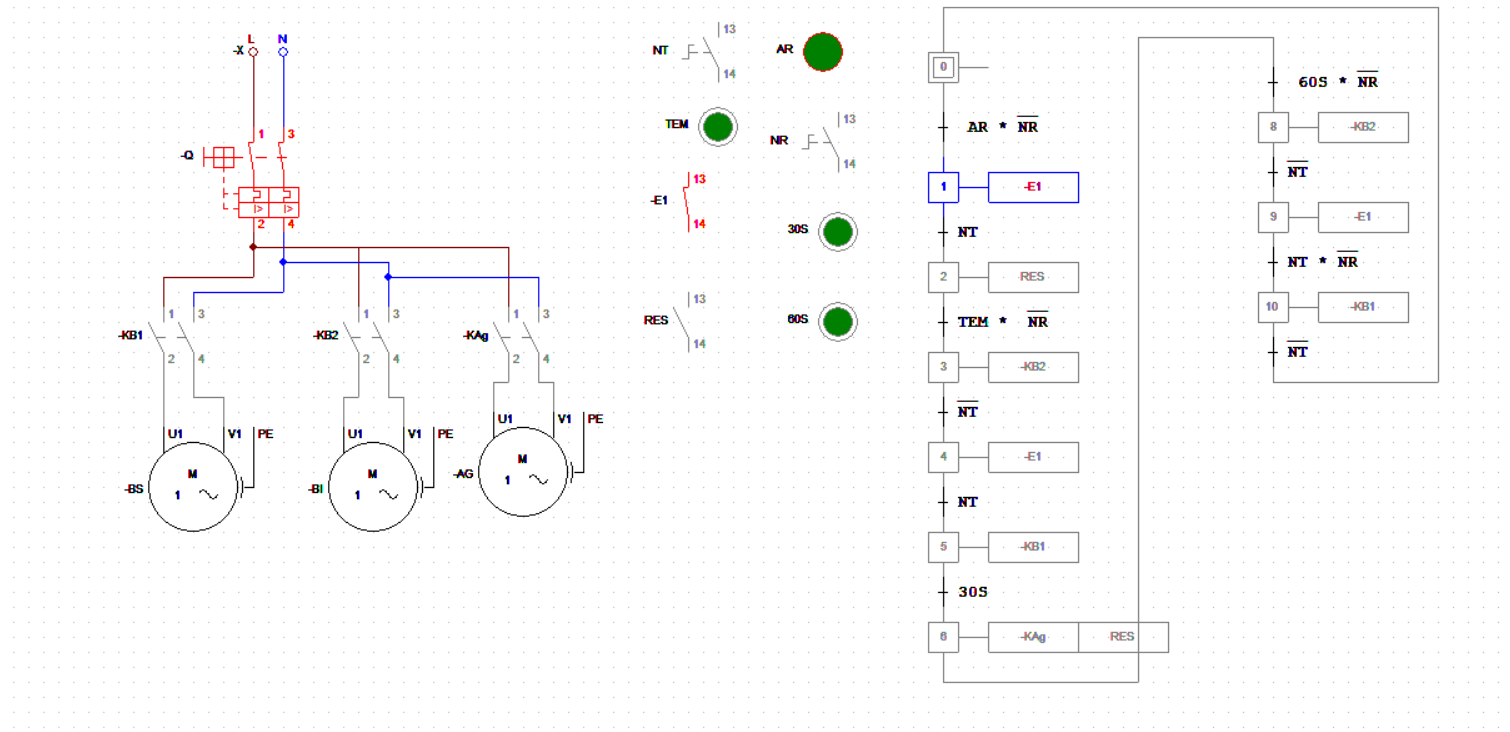
\includegraphics[width=\textwidth]{etapa-01.png}}{\fbox{\parbox[c][4cm][c]{1.0\textwidth}{\centering Inserte la imagen de la etapa 1}}}
\captionof{figure}{Etapa 1: Llenado de la cabina de operaciones.}\label{fig:etapa-01}
\end{minipage}\hfill
\begin{minipage}[t]{0.47\textwidth}
\raggedright\textbf{Etapa 2. Al llegar al nivel de referencia se acciona la resistencia de inmersión para calentar el agua hasta la temperatura de consigna.}\\[2mm]
\IfFileExists{figuras/etapa-02.png}{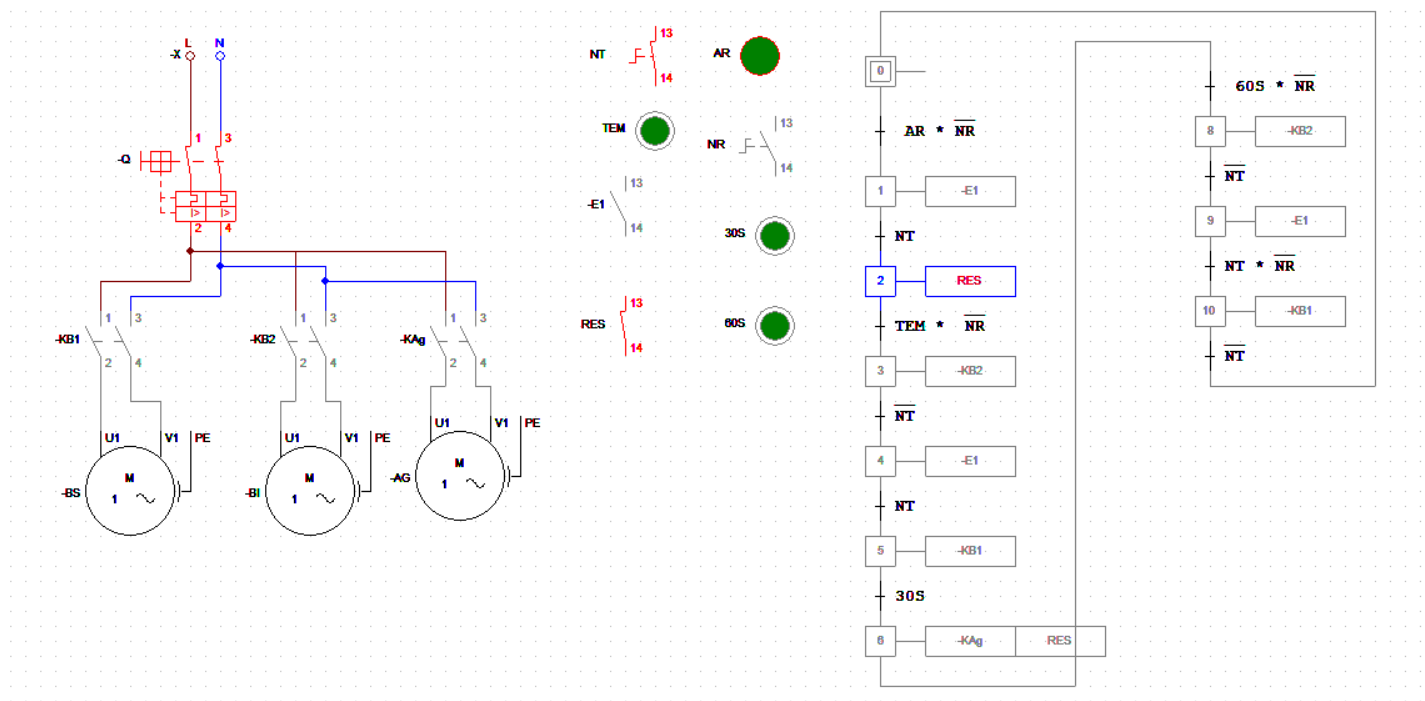
\includegraphics[width=\textwidth]{etapa-02.png}}{\fbox{\parbox[c][4cm][c]{0.9\textwidth}{\centering Inserte la imagen de la etapa 2}}}
\captionof{figure}{Etapa 2: Calentamiento del agua mediante resistencia de inmersión.}\label{fig:etapa-02}
\end{minipage}
\end{figure}

\begin{figure}[H]
\centering
\begin{minipage}[t]{0.47\textwidth}
\raggedright\textbf{Etapa 3. Al cumplirse la condición de calentamiento se acciona la bomba de drenado de la cabina, que lleva el agua de preenjuague a la tubería a limpiar, siempre que el tanque de agua residual tenga capacidad para no desbordarse.}\\[2mm]
\IfFileExists{figuras/etapa-03.png}{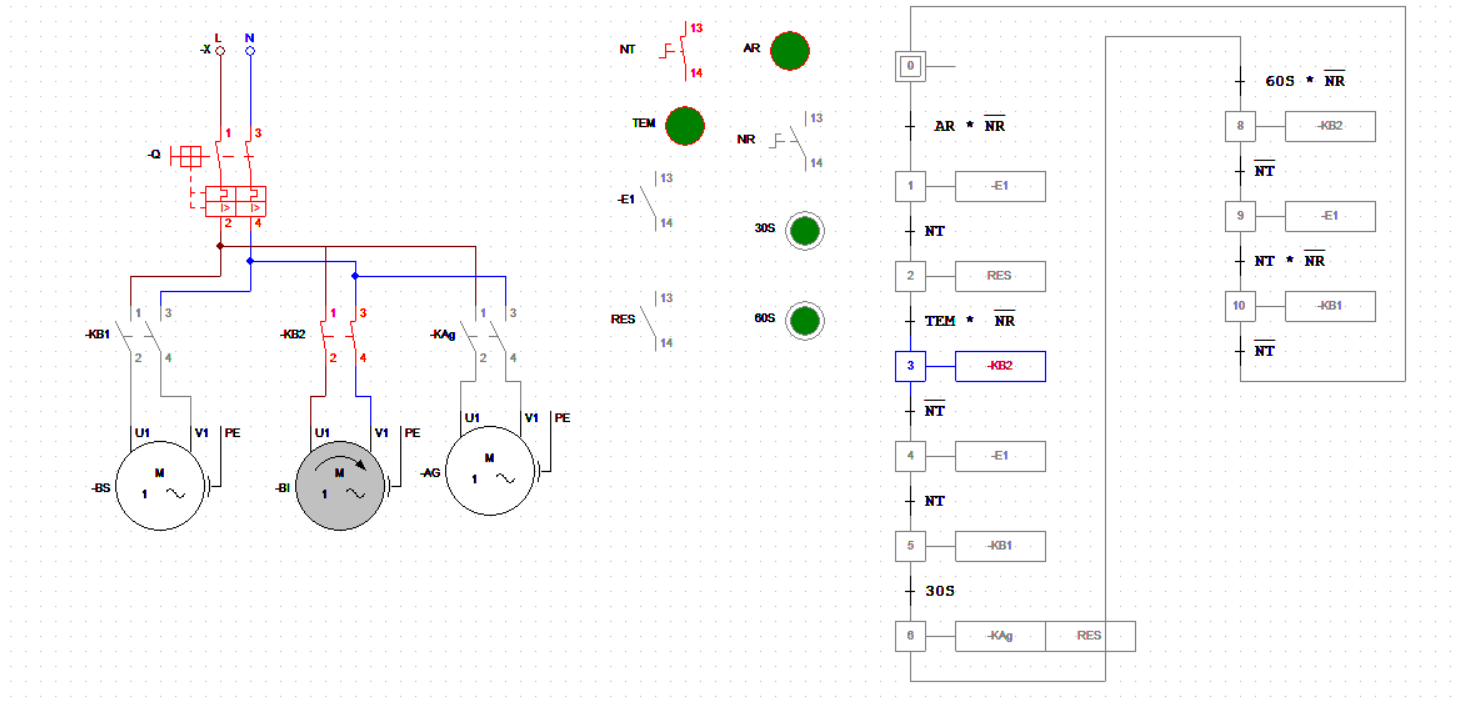
\includegraphics[width=\textwidth]{etapa-03.png}}{\fbox{\parbox[c][4cm][c]{0.9\textwidth}{\centering Inserte la imagen de la etapa 3}}}
\captionof{figure}{Etapa 3: Bomba de drenado de la cabina de operaciones.}\label{fig:etapa-03}
\end{minipage}\hfill
\begin{minipage}[t]{0.47\textwidth}
\raggedright\textbf{Etapa 4. Se realiza el rellenado de la cabina de operaciones cuando el nivel del tanque se detecta como bajo.}\\[2mm]
\IfFileExists{figuras/etapa-04.png}{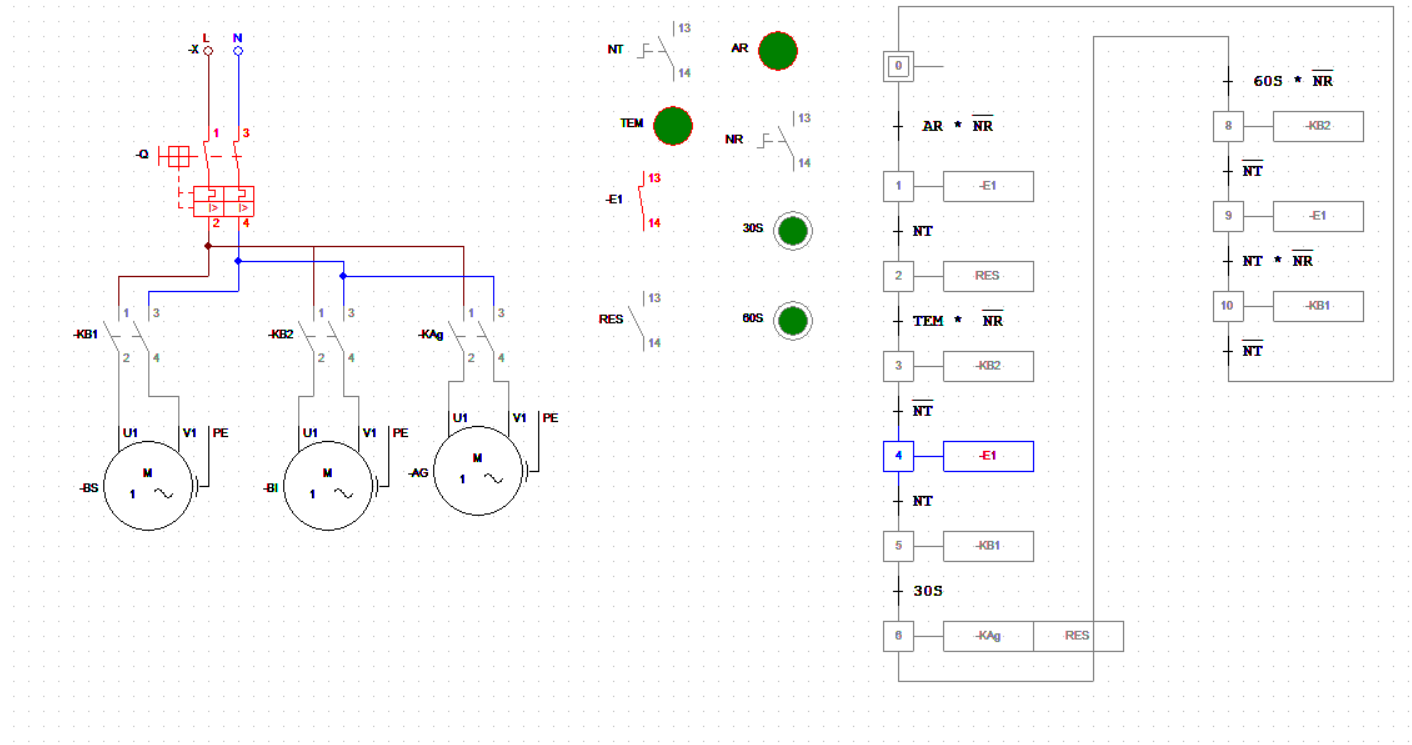
\includegraphics[width=\textwidth]{etapa-04.png}}{\fbox{\parbox[c][4cm][c]{0.9\textwidth}{\centering Inserte la imagen de la etapa 4}}}
\captionof{figure}{Etapa 4: Rellenado de la cabina de operaciones.}\label{fig:etapa-04}
\end{minipage}
\end{figure}

\begin{figure}[H]
\centering
\begin{minipage}[t]{0.47\textwidth}
\raggedright\textbf{Etapa 5. Con el tanque lleno se acciona la bomba de dosificación de la sustancia de limpieza.}\\[2mm]
\IfFileExists{figuras/etapa-05.png}{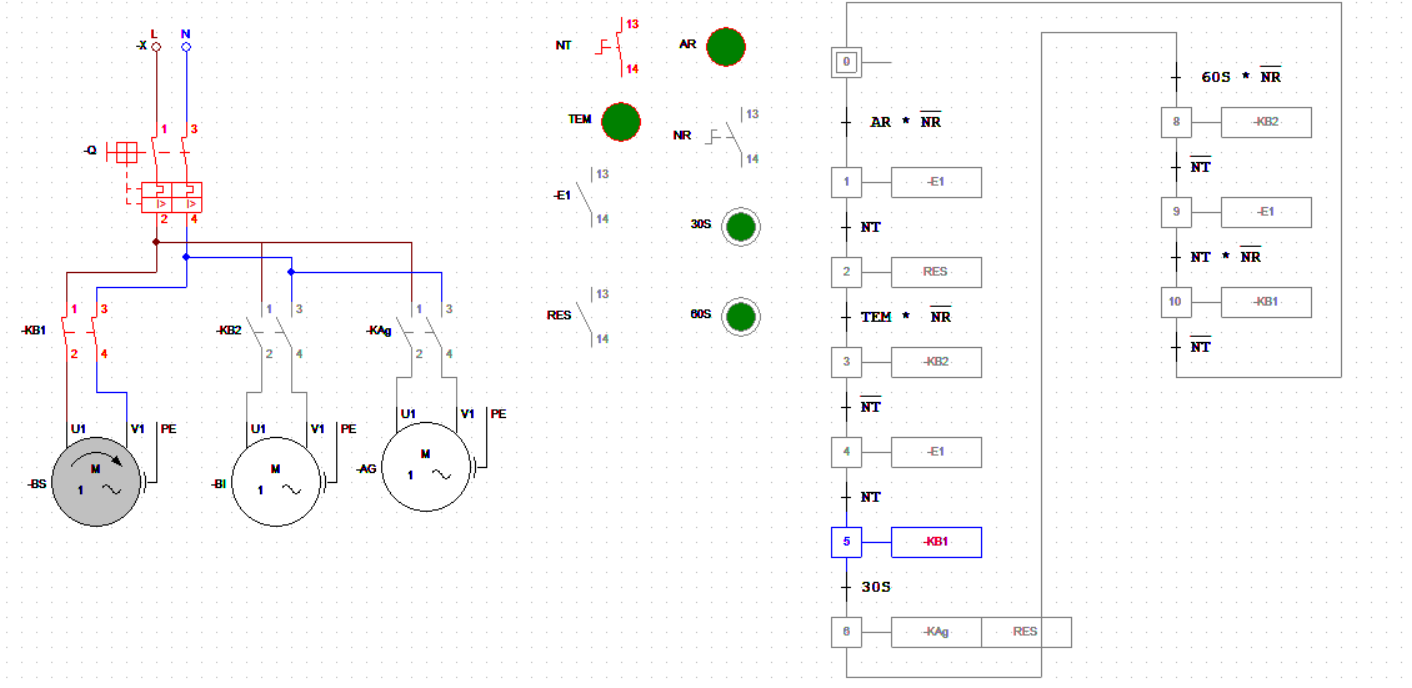
\includegraphics[width=\textwidth]{etapa-05.png}}{\fbox{\parbox[c][4cm][c]{0.9\textwidth}{\centering Inserte la imagen de la etapa 5}}}
\captionof{figure}{Etapa 5: Dosificación del jabón.}\label{fig:etapa-05}
\end{minipage}\hfill
\begin{minipage}[t]{0.47\textwidth}
\raggedright\textbf{Etapa 6. Tras el tiempo de accionamiento de la bomba de dosificación, se realizan la agitación y el calentamiento de la mezcla de agua y sustancia de limpieza.}\\[2mm]
\IfFileExists{figuras/etapa-06.png}{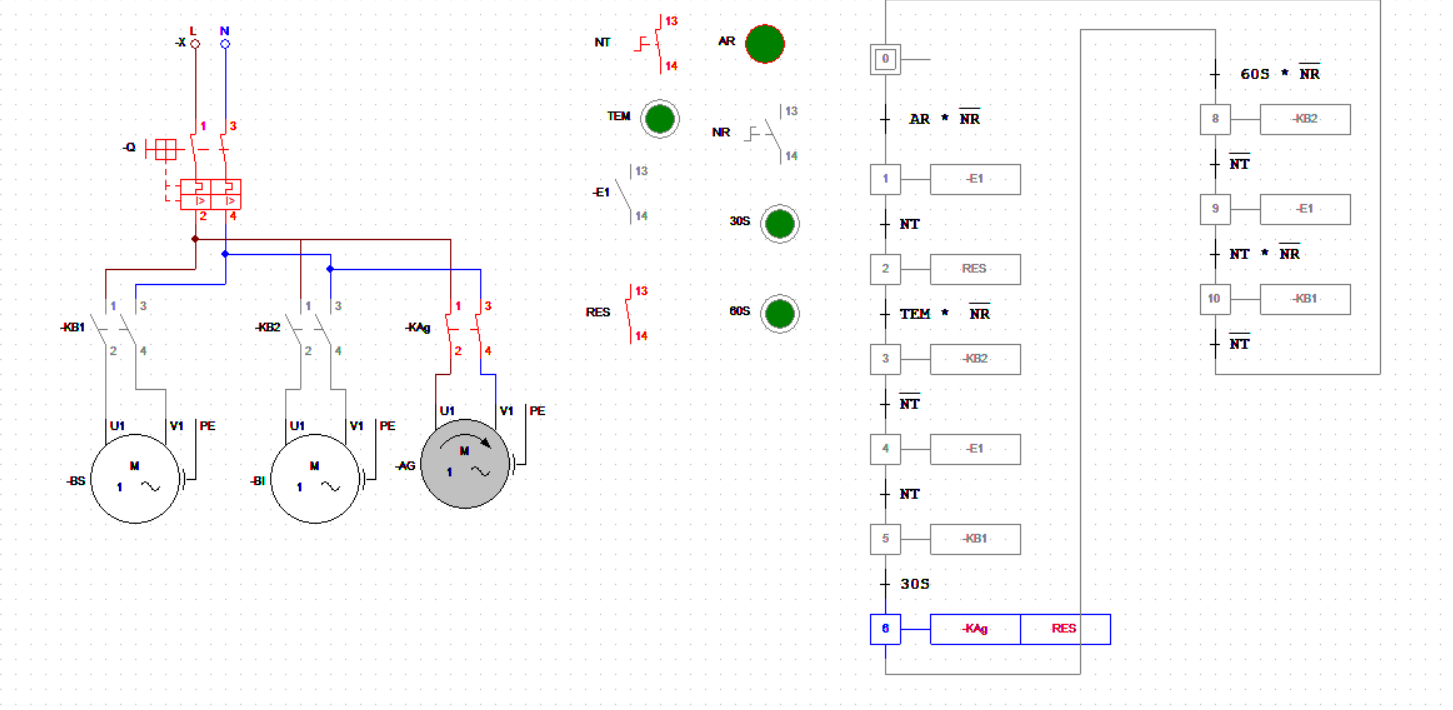
\includegraphics[width=\textwidth]{etapa-06.png}}{\fbox{\parbox[c][4cm][c]{0.9\textwidth}{\centering Inserte la imagen de la etapa 6}}}
\captionof{figure}{Etapa 6: Agitación y calentamiento de la mezcla de agua y sustancia de limpieza.}\label{fig:etapa-06}
\end{minipage}
\end{figure}
\begin{figure}[H]
\centering
\begin{minipage}[t]{0.47\textwidth}
\raggedright\textbf{Etapa 7. Tras calentar y agitar durante un tiempo determinado, y si el tanque de agua residual se encuentra en un nivel aceptable, se drena la cabina de operaciones hacia la tubería a limpiar.}\\[2mm]
\IfFileExists{figuras/etapa-07.png}{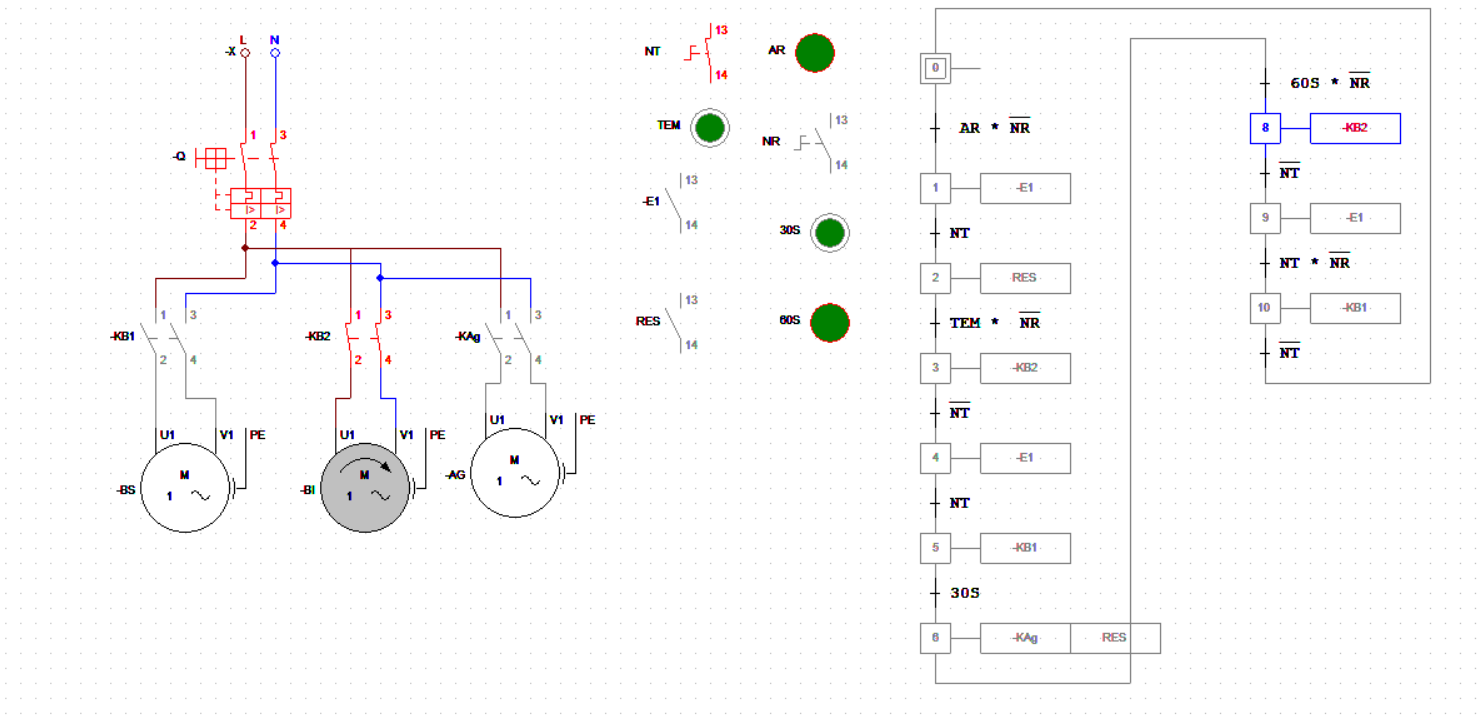
\includegraphics[width=\textwidth]{etapa-07.png}}{\fbox{\parbox[c][4cm][c]{0.9\textwidth}{\centering Inserte la imagen de la etapa 7}}}
\captionof{figure}{Etapa 7: Circulación de la solución de limpieza en la tubería.}\label{fig:etapa-07}
\end{minipage}\hfill
\begin{minipage}[t]{0.47\textwidth}
\raggedright\textbf{Etapa 8. Después de drenar la mezcla, y si el nivel del tanque es aceptable, se rellena el tanque para el último ciclo.}\\[2mm]
\IfFileExists{figuras/etapa-08.png}{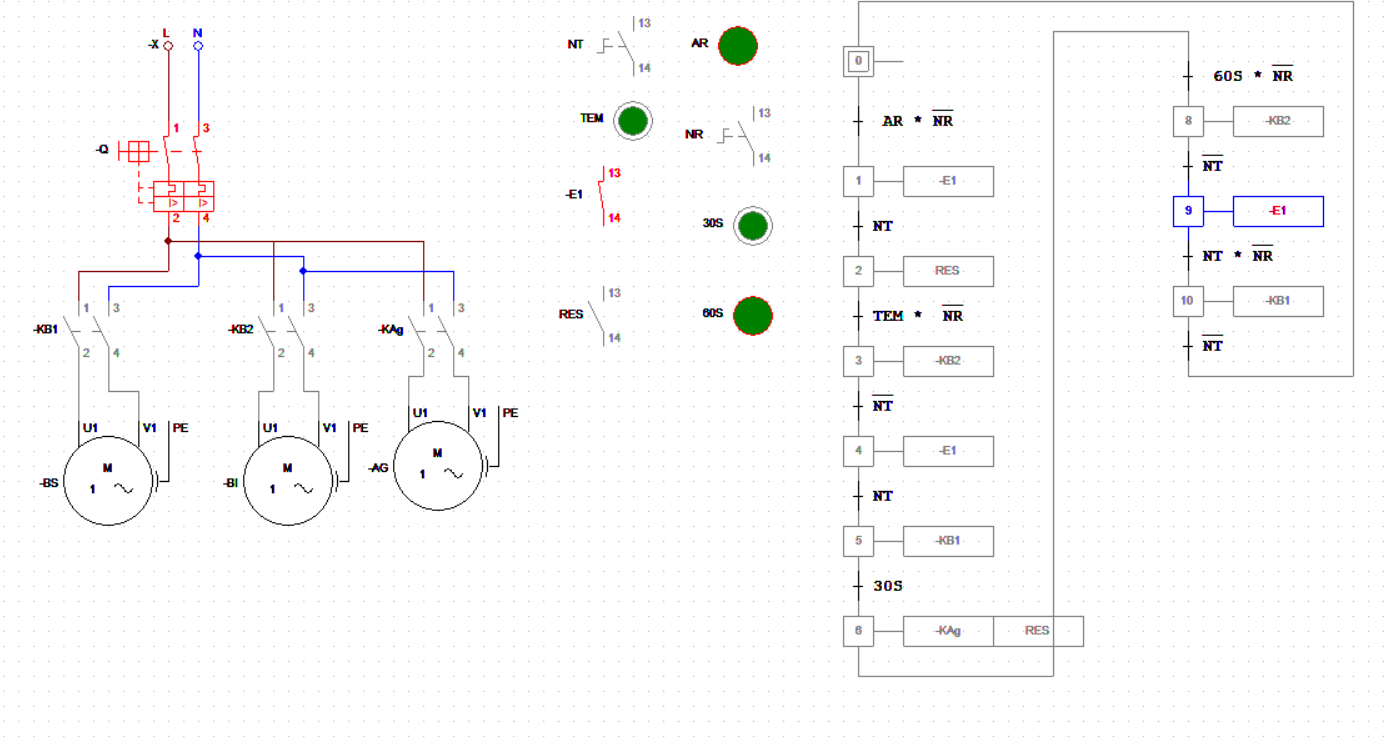
\includegraphics[width=\textwidth]{etapa-08.png}}{\fbox{\parbox[c][4cm][c]{0.9\textwidth}{\centering Inserte la imagen de la etapa 8}}}
\captionof{figure}{Etapa 8: Rellenado del tanque para el último ciclo.}\label{fig:etapa-08}
\end{minipage}
\end{figure}
\begin{figure}[H]
\centering
\begin{minipage}[t]{0.47\textwidth}
\raggedright\textbf{Etapa 9. Se realiza el enjuague con agua para eliminar los residuos remanentes.}\\[2mm]
\IfFileExists{figuras/etapa-09.png}{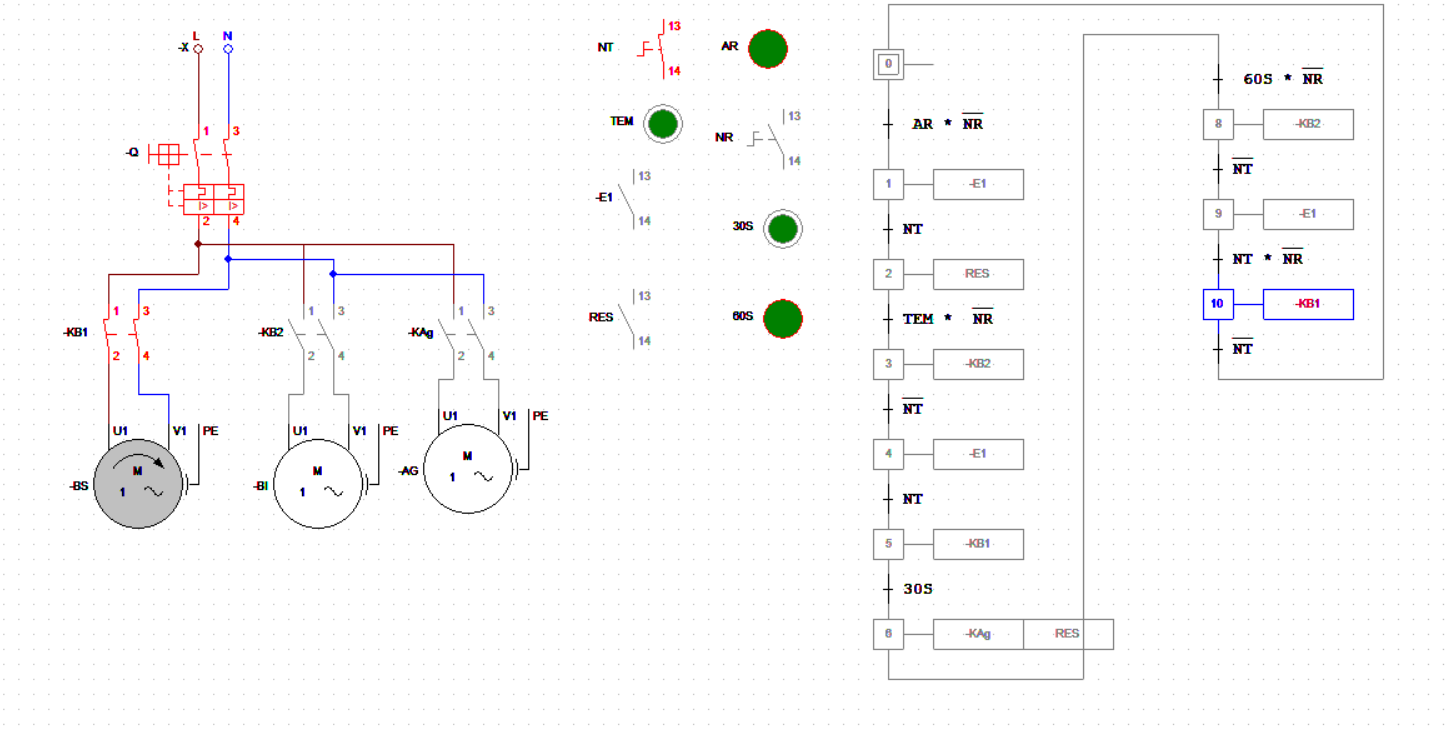
\includegraphics[width=\textwidth]{etapa-09.png}}{\fbox{\parbox[c][4cm][c]{0.9\textwidth}{\centering Inserte la imagen de la etapa 9}}}
\captionof{figure}{Etapa 9: Enjuague con agua para eliminar residuos remanentes.}\label{fig:etapa-09}
\end{minipage}\hfill
\end{figure}

\subsection{P\&ID y recorrido del fluido}
La Figura~\ref{fig:pid} presenta el P\&ID del sistema, actualizado con los elementos del prototipo del segundo corte, y la Tabla~\ref{tab:pid_elementos} identifica cada equipo, válvula, instrumento y línea. La simbología e identificación de los instrumentos sigue la norma ANSI/ISA-5.1 \cite{isa51_2009}: la primera letra del tag indica la variable medida o iniciadora y las siguientes, la función; los instrumentos de campo se representan con un círculo y las funciones implementadas en el PLC, con un rombo dentro de un cuadrado. Las válvulas on/off accionadas por la secuencia se identifican con la letra X (XV-102 y XV-103), y la secuencia del ciclo, con la función KC-100. Los símbolos de los equipos siguen la norma ISO~10628-2 \cite{iso10628_2}, y cada línea se designa como diámetro--servicio--número--material.

El recorrido del fluido sigue el esquema de paso único: el agua de red ingresa al tanque de mezcla TK-102 por la manguera 3/4"-AG-002-MG, a través de XV-102, y en la fase de lavado la bomba P-101 agrega el detergente desde TK-101 por la línea DT-001. Una vez preparado, el fluido sale de TK-102 por la línea 3/4"-PR-003-PVC, atraviesa XV-103 y es impulsado por P-102 hacia la tubería de prueba por la línea 1"-PR-004-PVC; el efluente llega a TK-103 por la línea EF-005 y, entre fases, se vacía manualmente al desagüe por la línea EF-006 mediante la válvula HV-101. En el lazo de temperatura, el elemento TE-101 (PT100) y el transmisor TT-101 entregan la medición al controlador TIC-101 del PLC, que acciona la resistencia E-101 a través del relé de estado sólido TY-101.

\begin{figure}[H]
\centering
\resizebox{\textwidth}{!}{% P&ID del sistema CIP portátil (prototipo del segundo corte).
% Requiere: \usetikzlibrary{arrows.meta,decorations.pathmorphing} y el color AzulUSTA.
\begin{tikzpicture}[
  font=\footnotesize,
  proceso/.style={line width=0.8pt,-{Stealth[length=2.2mm]}},
  tramo/.style={line width=0.8pt},
  senal/.style={AzulUSTA,dashed,line width=0.6pt},
  aplc/.style={AzulUSTA,font=\scriptsize},
  tag/.style={font=\footnotesize\bfseries},
  instrumento/.style={draw,circle,minimum size=0.9cm,inner sep=0pt,align=center,font=\scriptsize,fill=white},
  caja/.style={draw,rounded corners=3pt,align=center,fill=white,minimum height=0.7cm},
  tanque/.style={draw,line width=0.8pt,rounded corners=8pt,fill=white},
  solenoide/.pic={
    \draw[fill=white] (-0.35,-0.2)--(-0.35,0.2)--(0.35,-0.2)--(0.35,0.2)--cycle;
    \draw (0,0)--(0,0.35);
    \draw[fill=white] (-0.13,0.35) rectangle (0.13,0.61);
    \node[font=\tiny] at (0,0.48) {S};
  },
  manual/.pic={
    \draw[fill=white] (-0.35,-0.2)--(-0.35,0.2)--(0.35,-0.2)--(0.35,0.2)--cycle;
    \draw (0,0)--(0,0.35);
    \draw[line width=0.8pt] (-0.2,0.35)--(0.2,0.35);
  },
  centrifuga/.pic={
    \draw[fill=white] (0,0) circle (0.35);
    \draw (0,0.35)--(0.35,0.35);
    \draw (-0.2,-0.12)--(0.2,0)--(-0.2,0.12);
  },
  peristaltica/.pic={
    \draw[fill=white] (0,0) circle (0.35);
    \draw (0,0) circle (0.13);
    \foreach \a in {90,210,330} \fill (\a:0.24) circle (0.04);
  },
]

% ---------------- Tanques ----------------
\draw[tanque] (0,7.6) rectangle (1.8,9.8);
\node[align=center] at (0.9,8.7) {Tanque de\\detergente};
\node[tag] at (0.9,7.3) {TK-101};

\draw[tanque] (5.6,3.6) rectangle (9.4,7.4);
\node[align=center] at (7.5,6.95) {Tanque de mezcla};
\node[tag] at (7.5,7.65) {TK-102};

\draw[tanque] (14.8,3.8) rectangle (16.8,7.2);
\node[align=center] at (15.8,5.5) {Tanque de\\efluentes\\(30 L)};
\node[tag] at (15.8,7.45) {TK-103};

% ---------------- Línea L-1: detergente ----------------
\draw[tramo] (1.8,9.0)--(2.85,9.0);
\draw[proceso] (3.55,9.0)--(6.6,9.0)--(6.6,7.4);
\pic at (3.2,9.0) {peristaltica};
\node[tag] at (3.2,8.4) {P-101};
\draw[senal] (3.2,9.35)--(3.2,10.1) node[aplc,above] {a PLC};
\node at (5.0,9.25) {L-1};

% ---------------- Línea L-2: agua de red ----------------
\node[caja] (red) at (15.8,9.0) {Red de agua};
\draw[proceso] (red.west)--(8.4,9.0)--(8.4,7.4);
\pic at (12.3,9.0) {solenoide};
\node[tag] at (12.3,8.5) {SV-102};
\draw[senal] (12.3,9.61)--(12.3,10.1) node[aplc,above] {a PLC};
\node at (10.3,9.25) {L-2};

% ---------------- Instrumentos y elementos de TK-102 ----------------
% Resistencia de inmersión
\draw[tramo] (5.0,4.6)--(5.75,4.6);
\draw[line width=0.8pt,decorate,decoration={zigzag,segment length=4pt,amplitude=3pt}] (5.75,4.6)--(7.0,4.6);
\fill (5.0,4.6) circle (0.06);
\node[tag] at (5.0,4.25) {E-101};
\draw[senal] (4.94,4.6)--(3.4,4.6) node[aplc,left] {a PLC (SSR)};

% Transmisor de temperatura
\node[instrumento] (tt) at (4.4,6.0) {TT\\101};
\draw[tramo] (tt.east)--(6.3,6.0);
\draw[senal] (tt.west)--(3.4,6.0) node[aplc,left] {a PLC (4--20\,mA)};

% Interruptores de nivel alto y bajo
\node[instrumento] (lsh) at (10.6,6.8) {LSH\\101};
\draw[tramo] (lsh.west)--(8.95,6.8);
\draw[fill=white] (8.85,6.8) circle (0.1);
\draw[senal] (lsh.east)--(11.7,6.8) node[aplc,right] {a PLC};

\node[instrumento] (lsl) at (10.6,4.4) {LSL\\101};
\draw[tramo] (lsl.west)--(8.95,4.4);
\draw[fill=white] (8.85,4.4) circle (0.1);
\draw[senal] (lsl.east)--(11.7,4.4) node[aplc,right] {a PLC};

% Bomba de agitación sumergible
\pic[scale=0.75] at (7.9,4.15) {centrifuga};
\node[tag] at (7.9,4.75) {P-103};
\draw[-{Stealth[length=1.5mm]},line width=0.5pt] (8.45,3.95) arc (-60:200:0.2);
\draw[senal] (7.9,3.89)--(7.9,3.25)--(11.0,3.25) node[aplc,right] {a PLC (relé)};

% ---------------- Línea L-3: descarga e impulsión ----------------
\draw[tramo] (7.5,3.6)--(7.5,1.5)--(10.05,1.5);
\node at (7.15,2.55) {L-3};
\pic at (8.8,1.5) {solenoide};
\node[tag] at (8.8,1.0) {SV-103};
\draw[senal] (8.8,2.11)--(8.8,2.5) node[aplc,above] {a PLC};

\pic at (10.4,1.5) {centrifuga};
\node[tag] at (10.25,2.3) {P-102};
\draw[senal] (10.4,1.15)--(10.4,0.55);
\node[aplc] at (10.4,0.35) {a PLC (SSR)};

\node[caja,minimum width=2.4cm] (tub) at (12.65,1.85) {Tubería de prueba};
\draw[tramo] (10.75,1.85)--(tub.west);

% ---------------- Línea L-4: efluente ----------------
\draw[proceso] (tub.east)--(14.2,1.85)--(14.2,6.6)--(14.8,6.6);
\node at (13.85,4.5) {L-4};

% ---------------- Línea L-5: vaciado manual ----------------
\node[caja] (des) at (15.8,0.9) {Desagüe};
\draw[proceso] (15.8,3.8)--(des.north);
\pic[rotate=-90] at (15.8,2.55) {manual};
\node[tag,right] at (16.15,2.65) {HV-101};
\node[font=\scriptsize,right] at (16.15,2.25) {(manual)};
\node at (15.45,3.3) {L-5};

% ---------------- Convenciones ----------------
\draw[line width=0.8pt] (0,2.0)--(0.8,2.0);
\node[right] at (0.9,2.0) {Línea de proceso};
\draw[senal] (0,1.5)--(0.8,1.5);
\node[right] at (0.9,1.5) {Señal eléctrica PLC};
\node[right,font=\scriptsize,align=left] at (0,0.9) {Esquema de paso único:\\sin recirculación hacia TK-102};

\end{tikzpicture}
}
\caption{P\&ID del sistema CIP portátil.}
\label{fig:pid}
\end{figure}

\newlength{\anchoflexpid}
\setlength{\anchoflexpid}{\dimexpr\textwidth-2.5cm-3.5cm-3.0cm-8\tabcolsep\relax}

\begin{scriptsize}
\begin{longtable}{L{2.5cm}L{3.5cm}L{3.0cm}L{\anchoflexpid}}
\caption{Identificación de elementos del diagrama P\&ID (Equipos, Válvulas, Instrumentos y Líneas).}\label{tab:pid_elementos} \\
\toprule
\textbf{Tag / Identificador} & \textbf{Nombre} & \textbf{Categoría / Tipo} & \textbf{Función} \\
\midrule
\endfirsthead

\multicolumn{4}{l}{\small \tablename\ \thetable{} -- continuación}\\
\toprule
\textbf{Tag / Identificador} & \textbf{Nombre} & \textbf{Categoría / Tipo} & \textbf{Función} \\
\midrule
\endhead

\midrule
\multicolumn{4}{r}{\small Continúa en la siguiente página}\\
\endfoot

\bottomrule
\endlastfoot

TK-101 & Tanque de detergente & Equipo (Tanque) & Almacena el detergente antes de la dosificación. \\
P-101 & Bomba dosificadora peristáltica & Equipo (Bomba) & Agrega el detergente desde TK-101 al tanque de mezcla durante la fase de lavado. \\
TK-102 & Tanque de mezcla & Equipo (Tanque) & Tanque de plástico de 50\,L donde se prepara y calienta el fluido de cada fase. \\
P-103 & Bomba de agitación sumergible & Equipo (Bomba) & Homogeniza la mezcla dentro de TK-102 antes del calentamiento. \\
E-101 & Resistencia de inmersión & Equipo (Calefactor) & Calienta el fluido en TK-102 hasta la consigna. \\
P-102 & Bomba de impulsión & Equipo (Bomba) & Impulsa el fluido desde TK-102 hacia la tubería de prueba. \\
TK-103 & Tanque de efluentes & Equipo (Tanque) & Tanque metálico de 30\,L que recoge el efluente de la tubería de prueba. \\
SV-102 & Electroválvula de llenado & Válvula de control & Permite o interrumpe el ingreso de agua de red al tanque de mezcla. \\
SV-103 & Electroválvula de descarga & Válvula de control & Permite o interrumpe la salida del fluido de TK-102 hacia la bomba P-102. \\
HV-101 & Válvula manual de vaciado & Válvula manual & Permite vaciar TK-103 al desagüe entre fases. \\
LSL-101 & Interruptor de nivel bajo & Instrumento & Detecta el nivel bajo en TK-102; detiene la bomba de impulsión al vaciarse el tanque. \\
LSH-101 & Interruptor de nivel alto & Instrumento & Detecta el nivel alto en TK-102; termina el llenado. \\
TT-101 & Transmisor de temperatura & Instrumento & Mide la temperatura del fluido en TK-102 (PT100 con salida de 4--20\,mA). \\
L-1 & Línea de detergente & Tubería de proceso & Conduce el detergente desde TK-101 hacia TK-102. \\
L-2 & Línea de agua & Tubería de proceso & Alimenta agua de red a TK-102. \\
L-3 & Línea de descarga & Tubería de proceso & Conduce el fluido desde la base de TK-102 hacia SV-103 y P-102. \\
L-4 & Línea de efluente & Tubería de proceso & Conduce el efluente desde la tubería de prueba hasta TK-103. \\
L-5 & Línea de vaciado & Tubería de proceso & Conduce el contenido de TK-103 al desagüe a través de HV-101. \\
--- & Señales de control (PLC) & Línea de instrumentación & Transmite las señales de entrada y salida entre el PLC y los equipos e instrumentos (SV-102, SV-103, P-101, P-102, P-103, E-101, TT-101, LSL-101 y LSH-101). \\

\end{longtable}
\end{scriptsize}

\subsection{Estructura y distribución}
El prototipo se construyó sobre dos carros móviles, cuyas bases tienen casi las mismas dimensiones: 1000 × 500\,mm, fabricadas en tubo cuadrado de 40 × 40 × 4\,mm, con zonas para ruedas en las esquinas y una placa de 1000 × 500\,mm como superficie de apoyo (Figura~\ref{fig:plano_bases}). Las dos bases solo difieren en la altura de la barra donde se ubican las ruedas: en el carro del PLC esta altura es de 50\,mm, para que la barra pueda adaptarse al unirse con el otro carro. La unión entre los dos carros queda pendiente y se resolverá con un producto comercial que se adapte.

\insertarfigura{plano_bases.jpg}{Plano de las bases de los carros.}{fig:plano_bases}

El primer carro soporta los tanques y el circuito hidráulico. Sobre su base se instala una estructura de soporte de 780 × 460\,mm en planta, con alojamientos de 200\,mm y 500\,mm de altura para los tanques (Figura~\ref{fig:plano_soporte_tanques}). Las dimensiones de los alojamientos priorizan una tolerancia positiva, de modo que se garantice el ajuste y montaje correctos de los tanques.

\insertarfigura{plano_soporte_tanques.jpg}{Plano de la estructura de soporte de los tanques.}{fig:plano_soporte_tanques}

El segundo carro aloja el PLC, el panel HMI y el tablero eléctrico, e incorpora un banco para relés y demás elementos del tablero, de 340 × 300 × 370\,mm, elaborado con perfiles de 20 × 20 × 2\,mm (Figura~\ref{fig:plano_banco_reles}). La estructura se diseñó para que el sistema pueda transportarse en un vehículo, pasar por puertas y ascensores y mantenerse estable durante la operación.

\insertarfigura[0.8\textwidth]{plano_banco_reles.jpg}{Plano del banco para relés del carro del PLC.}{fig:plano_banco_reles}

\subsection{Equipo o circuito de prueba}
El circuito de prueba está conformado por una tubería de PVC de una pulgada de diámetro nominal y una longitud aproximada de 6\,m (REQ-05), representativa de una línea de proceso de pequeña escala. Su entrada se conecta a la descarga de la bomba de impulsión P-102 y su salida conduce el efluente al tanque de efluentes TK-103, de modo que el agua de preenjuague, la solución de limpieza y el agua de enjuague final se recogen sin vertimientos sobre el área de trabajo. Entre fases, el operario vacía TK-103 al drenaje mediante la válvula manual HV-101.

Durante cada ensayo se registrarán el tiempo de cada fase, la temperatura alcanzada en las fases con calentamiento y el estado de los interruptores de nivel, y se verificarán la estanqueidad de las conexiones y el funcionamiento de las electroválvulas y de las bombas. Ante una fuga o el accionamiento de la parada de emergencia, el sistema deberá interrumpir el llenado y la impulsión del fluido de manera segura.

\campo{Pendiente: método para evaluar la efectividad de la limpieza de la tubería de prueba.}
